\documentclass[main.tex]{subfiles}

\begin{document}

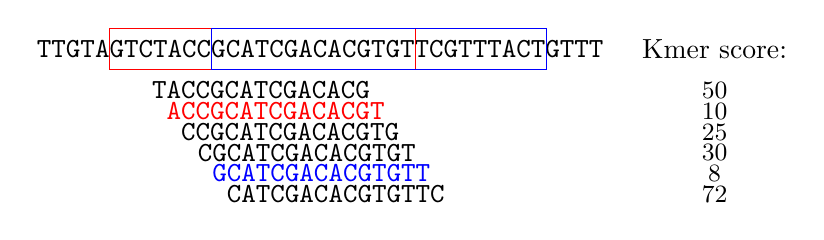
\begin{tikzpicture}[x=0.75pt,y=0.75pt,yscale=-1,xscale=1]

\draw (10, 10) node {\texttt{TTGTAGTCTACCGCATCGACACGTGTTCGTTTACTGTTT}};

%\draw [color=blue] (-109, 0) -- (-109, 20);
%\draw [color=purple] (-102, 0) -- (-102, 20);
%\draw [color=purple] (-95, 0) -- (-95, 20);

\draw [color=red] (-91.5, 0) rectangle (56, 20);
\draw [color=blue] (-42.5, 0) rectangle (119, 20);
\draw (-18.5, 30) node {\texttt{TACCGCATCGACACG}};
\draw (-11.5, 40) node {\texttt{\color{red}ACCGCATCGACACGT}};
\draw (-4.5, 50) node {\texttt{CCGCATCGACACGTG}};
\draw (3.5, 60) node {\texttt{CGCATCGACACGTGT}};
\draw (10.5, 70) node {\texttt{\color{blue}GCATCGACACGTGTT}};
\draw (17.5, 80) node {\texttt{CATCGACACGTGTTC}};

\draw (200, 10) node {Kmer score:};
\draw (200, 30) node {\small 50};
\draw (200, 40) node {\small 10};
\draw (200, 50) node {\small 25};
\draw (200, 60) node {\small 30};
\draw (200, 70) node {\small 8};
\draw (200, 80) node {\small 72};

\end{tikzpicture}

\end{document}